% Система archive-index. Кожне твердження перевірено за src/archive_index (рівень доказів L1: код і тести).
\section{Система archive-index}\label{sec:system}

\subsection{Архітектура і потік даних}
archive-index зберігає кожен архів в одній базі SQLite. Таблиця \code{documents} описує кожен файл-джерело (колекція, шлях, розмір, час зміни, SHA-256, назва, проєкт); таблиця \code{chunks} містить текстові фрагменти з локатором (сторінка, слайд, часове вікно, кадр), вектор вкладення у двійковому вигляді і геш тексту, з якого цей вектор отримано. Віртуальна таблиця FTS5 індексує три стовпці фрагмента: описані нижче словесні терми, текст і заголовок; токенізатор \code{unicode61} зберігає діакритику. База працює в режимі журналу попереднього запису (WAL), тож термінальний інтерфейс, заплановані запуски індексації та окремі пошуки читають базу, поки індексатор пише.

Джерела розподілено за колекціями: нотатки Markdown (\code{wiki}); офісні документи і PDF (\code{docs}; файли \code{.doc}, \code{.rtf}, \code{.odt}, \code{.ppt} та \code{.odp} конвертуються через LibreOffice); таблиці і CSV (\code{tables}); історія Git; сесії агентів Claude і Codex; журнали запусків; зображення; звук; відео. Вихідний код, конфігурації та журнали є колекціями за вибором: у них шукають, лише коли їх названо. Markdown ділиться за заголовками, а абзаци складаються у фрагменти до 1\,200 символів; довший абзац розрізається на цій межі.

\begin{figure}[p]
\centering
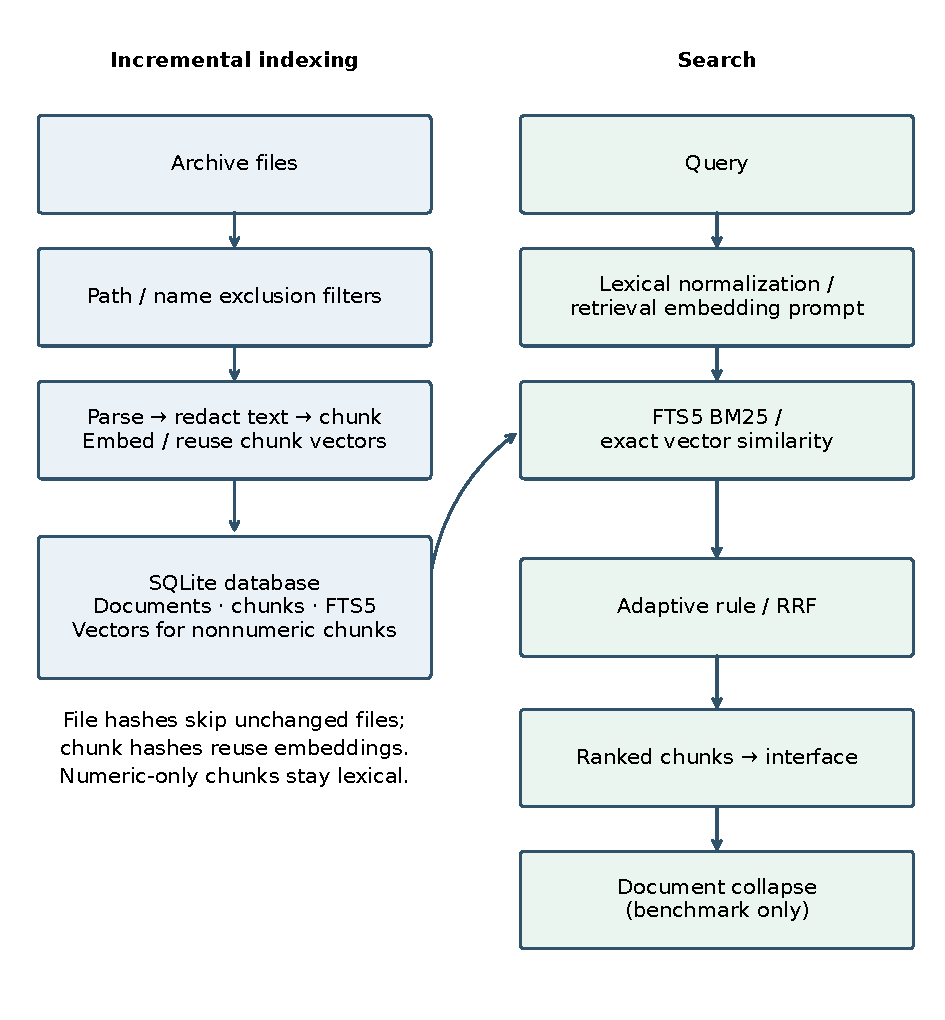
\includegraphics[width=\linewidth]{architecture.pdf}
\caption{Потік даних індексації й пошуку з типовим локальним бекендом. Редагування секретів застосовує відомі текстові шаблони; вміст зображень і звуку так не очищується. Числові фрагменти лишаються доступними лексичному пошуку без векторів. Згортання до документів належить бенчмарку й не входить у таймер запиту.}
\label{fig:architecture}
\end{figure}

\subsection{Лексичний рівень}
Слово --- це послідовність літер і цифр Юнікоду, яку можуть з'єднувати дефіс або апостроф, завдовжки щонайменше два символи, у нижньому регістрі. Чотири символи апострофа, що трапляються в українському тексті (U+2019, U+02BC, U+2018 і зворотний гравіс), до токенізації замінюються на апостроф ASCII, тож \emph{м’ята} і \emph{мʼята} --- одне слово. Стовпець \code{terms} зберігає кожне слово і його нормальні форми з українського та російського аналізаторів pymorphy3. Слово з літерою, що є лише в українській абетці (і, ї, є, ґ), проходить тільки український аналізатор; інші слова --- обидва. Якщо словник знає слово, зберігаються лише словникові нормальні форми; здогадки аналізаторів використовуються тільки для слів, яких не знає жоден словник (ваду, яку виправляє це правило, описано в додатку~\ref{sec:intro-history}).

Ідентифікатори на кшталт \code{36.101}, \code{19.6.0} чи \code{RVZ0014A-2} (послідовності літер і цифр, з'єднані крапками чи скісними рисками, або дефісом перед цифрою) шукаються як точні фрази, тож запит \code{36.109} ніколи не збігається з документом, що містить лише \code{36}. Запит стає виразом FTS5, у якому кожне слово --- диз'юнкція його поверхневої та нормальних форм, слова поєднано через OR, а умову ідентифікатора, якщо вона є, приєднано до слів через AND. Лексичне ранжування --- BM25 у FTS5.

\subsection{Семантичний рівень}
Семантичний рівень використовує EmbeddingGemma~2 через SentenceTransformers: у bfloat16 на GPU (картка моделі попереджає, що float16 погіршує вкладення) і у float32 на CPU. Документи кодуються як \code{title: <назва> | text: <фрагмент>}; запити отримують пошуковий промпт моделі \code{task: search result | query:}, а при пошуку в колекції коду --- \code{task: code retrieval | query:}. Вектори нормуються за L2; 256-вимірний варіант обрізає їх (матрьошкове обрізання) і нормує знову. Зображення, сторінки PDF без текстового шару і кадри відео (один раз на 5~с, не більше 120 на відео) кодуються як зображення в тому самому просторі. Звук передискретизується до 16~кГц і кодується вікнами по 20~с із кроком 15~с; якщо до запису додано файл розшифровки, рядки розшифровки, що перетинаються з вікном, стають його текстом. Сервер llama.cpp із GGUF-збіркою моделі --- необов'язковий суто текстовий бекенд. Семантичний пошук точний: усі вектори тримаються в пам'яті й оцінюються одним добутком матриці на вектор у NumPy, без індексу наближеного пошуку найближчих сусідів.

\subsection{Злиття}
Доступні три режими ранжування: лише лексичний, лише семантичний і гібридний. Типова гібридна стратегія (\sys{adaptive}) дивиться на найкращий лексичний фрагмент. Якщо він містить щонайменше 90\% слів запиту як окремі слова, запит вважається пошуком точної фрази: повертаються лише лексичні результати в порядку BM25, але фрагменти, де слова запиту йдуть по порядку з проміжком до трьох слів, переносяться наперед. Інакше спершу йде семантичне ранжування, а за ним --- лексичні результати, яких у ньому ще немає; без лексичного збігу результат суто семантичний. Альтернативна гібридна стратегія --- злиття за оберненими рангами (reciprocal rank fusion) з $k=60$ (\sys{rrf}). Інтерфейс показує щонайбільше три фрагменти документа і кількість решти; прогони бенчмарку згортають фрагменти до документів (розділ~\ref{sec:method}).

\subsection{Інкрементальна індексація}
Файл пропускається, якщо не змінилися розмір і час зміни, а також якщо не змінився SHA-256; лише інакше його розбирають знову. Вектори фрагментів, геш тексту яких уже збережено, використовуються повторно, тож після правки нотатки заново кодуються тільки змінені фрагменти. Зниклі файли видаляються зі своєї колекції. Фрагменти нотаток і документів, що мають менше 20 літер (номери сторінок, розділові знаки), відкидаються, якщо не всі фрагменти файлу такі короткі; зображення і звук не відкидаються ніколи. Кожен запуск записує звіт про проіндексовані, пропущені й невдалі файли; помилка в одному файлі не зупиняє запуску.

\subsection{Приватність}
Типовий бекенд вкладень обробляє вміст документів локально. Необов'язковий клієнт llama.cpp типово звертається до сервера через петльову адресу; зовнішня адреса у \code{ARCHIVE\_LLAMA\_URL} передає текст до цього вузла. Отже, локальність оброблення залежить від налаштування бекенду. Каталоги \code{.ssh}, \code{.gnupg}, \code{.aws}, \code{.kube}, \code{.password-store}, \code{.docker} і сховища ключів, а також файли, назви яких відповідають шаблонам ключів, сертифікатів, сховищ паролів, файлів оточення й облікових даних (наприклад, \code{*.pem}, \code{*.kdbx}, \code{id\_rsa*}, \code{.env}, \code{*secret*}, \code{*token*}), ніколи не потрапляють до індексу. У проіндексованому тексті блоки приватних ключів PEM, ключі доступу у форматах кількох поширених сервісів (OpenAI, AWS, GitHub, Slack, bearer-токени) та явні присвоєння облікових даних на зразок \code{password=...} замінюються міткою до збереження. Шаблони охоплюють лише відомі формати; це страховка, а не гарантія. Звіт про приховування рахує види і ніколи не зберігає значень.
